\section{Electronics}
\label{sec:electronics}
The circuit design is represented in figure \ref{fig:circuit-design}.
In this section we expose the electronic components used in the circuit.

\subsection{ESP32}
ESP32 is a series of low-cost, low-power system on a chip microcontroller with integrated Wi-Fi and dual-mode Bluetooth.
We've bought the ESP32 D1 R32, the one in figure \ref{fig:esp32}, for better attaching the motor using the CNC shield V3 (which is briefly explained in the following).

We decided to follow the "WeMos R32 and CNC V3" OnStep project (at \url{https://onstep.groups.io/g/main/wiki/19670}).
OnStep is an open source software providing the control of four stepper motors (RA, DEC, focuser and rotator for astrophotography), weather sensor handling, Wi-Fi and Bluetooth connection, polar alignment and other nice features.

\begin{figure*}
    \begin{minipage}[c][10cm][c]{0.35\textwidth}
        \centering
        \vspace*{\fill}
        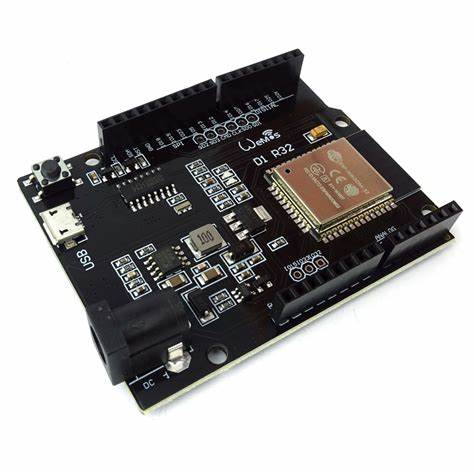
\includegraphics[scale=0.28]{esp32_d1_r32.jpg}
        \subcaption{ESP32 D1 R32 picture.}
        \label{fig:esp32}
        
        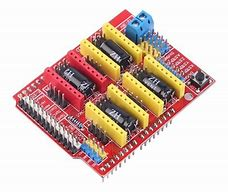
\includegraphics[scale=0.5]{CNC3.jpg}
        \subcaption{CNC3 Shield V3.}
        \label{fig:cnc3}
    \end{minipage}
    \begin{minipage}[c][10cm][t]{0.5\textwidth}
        \vspace*{\fill}
        \centering
        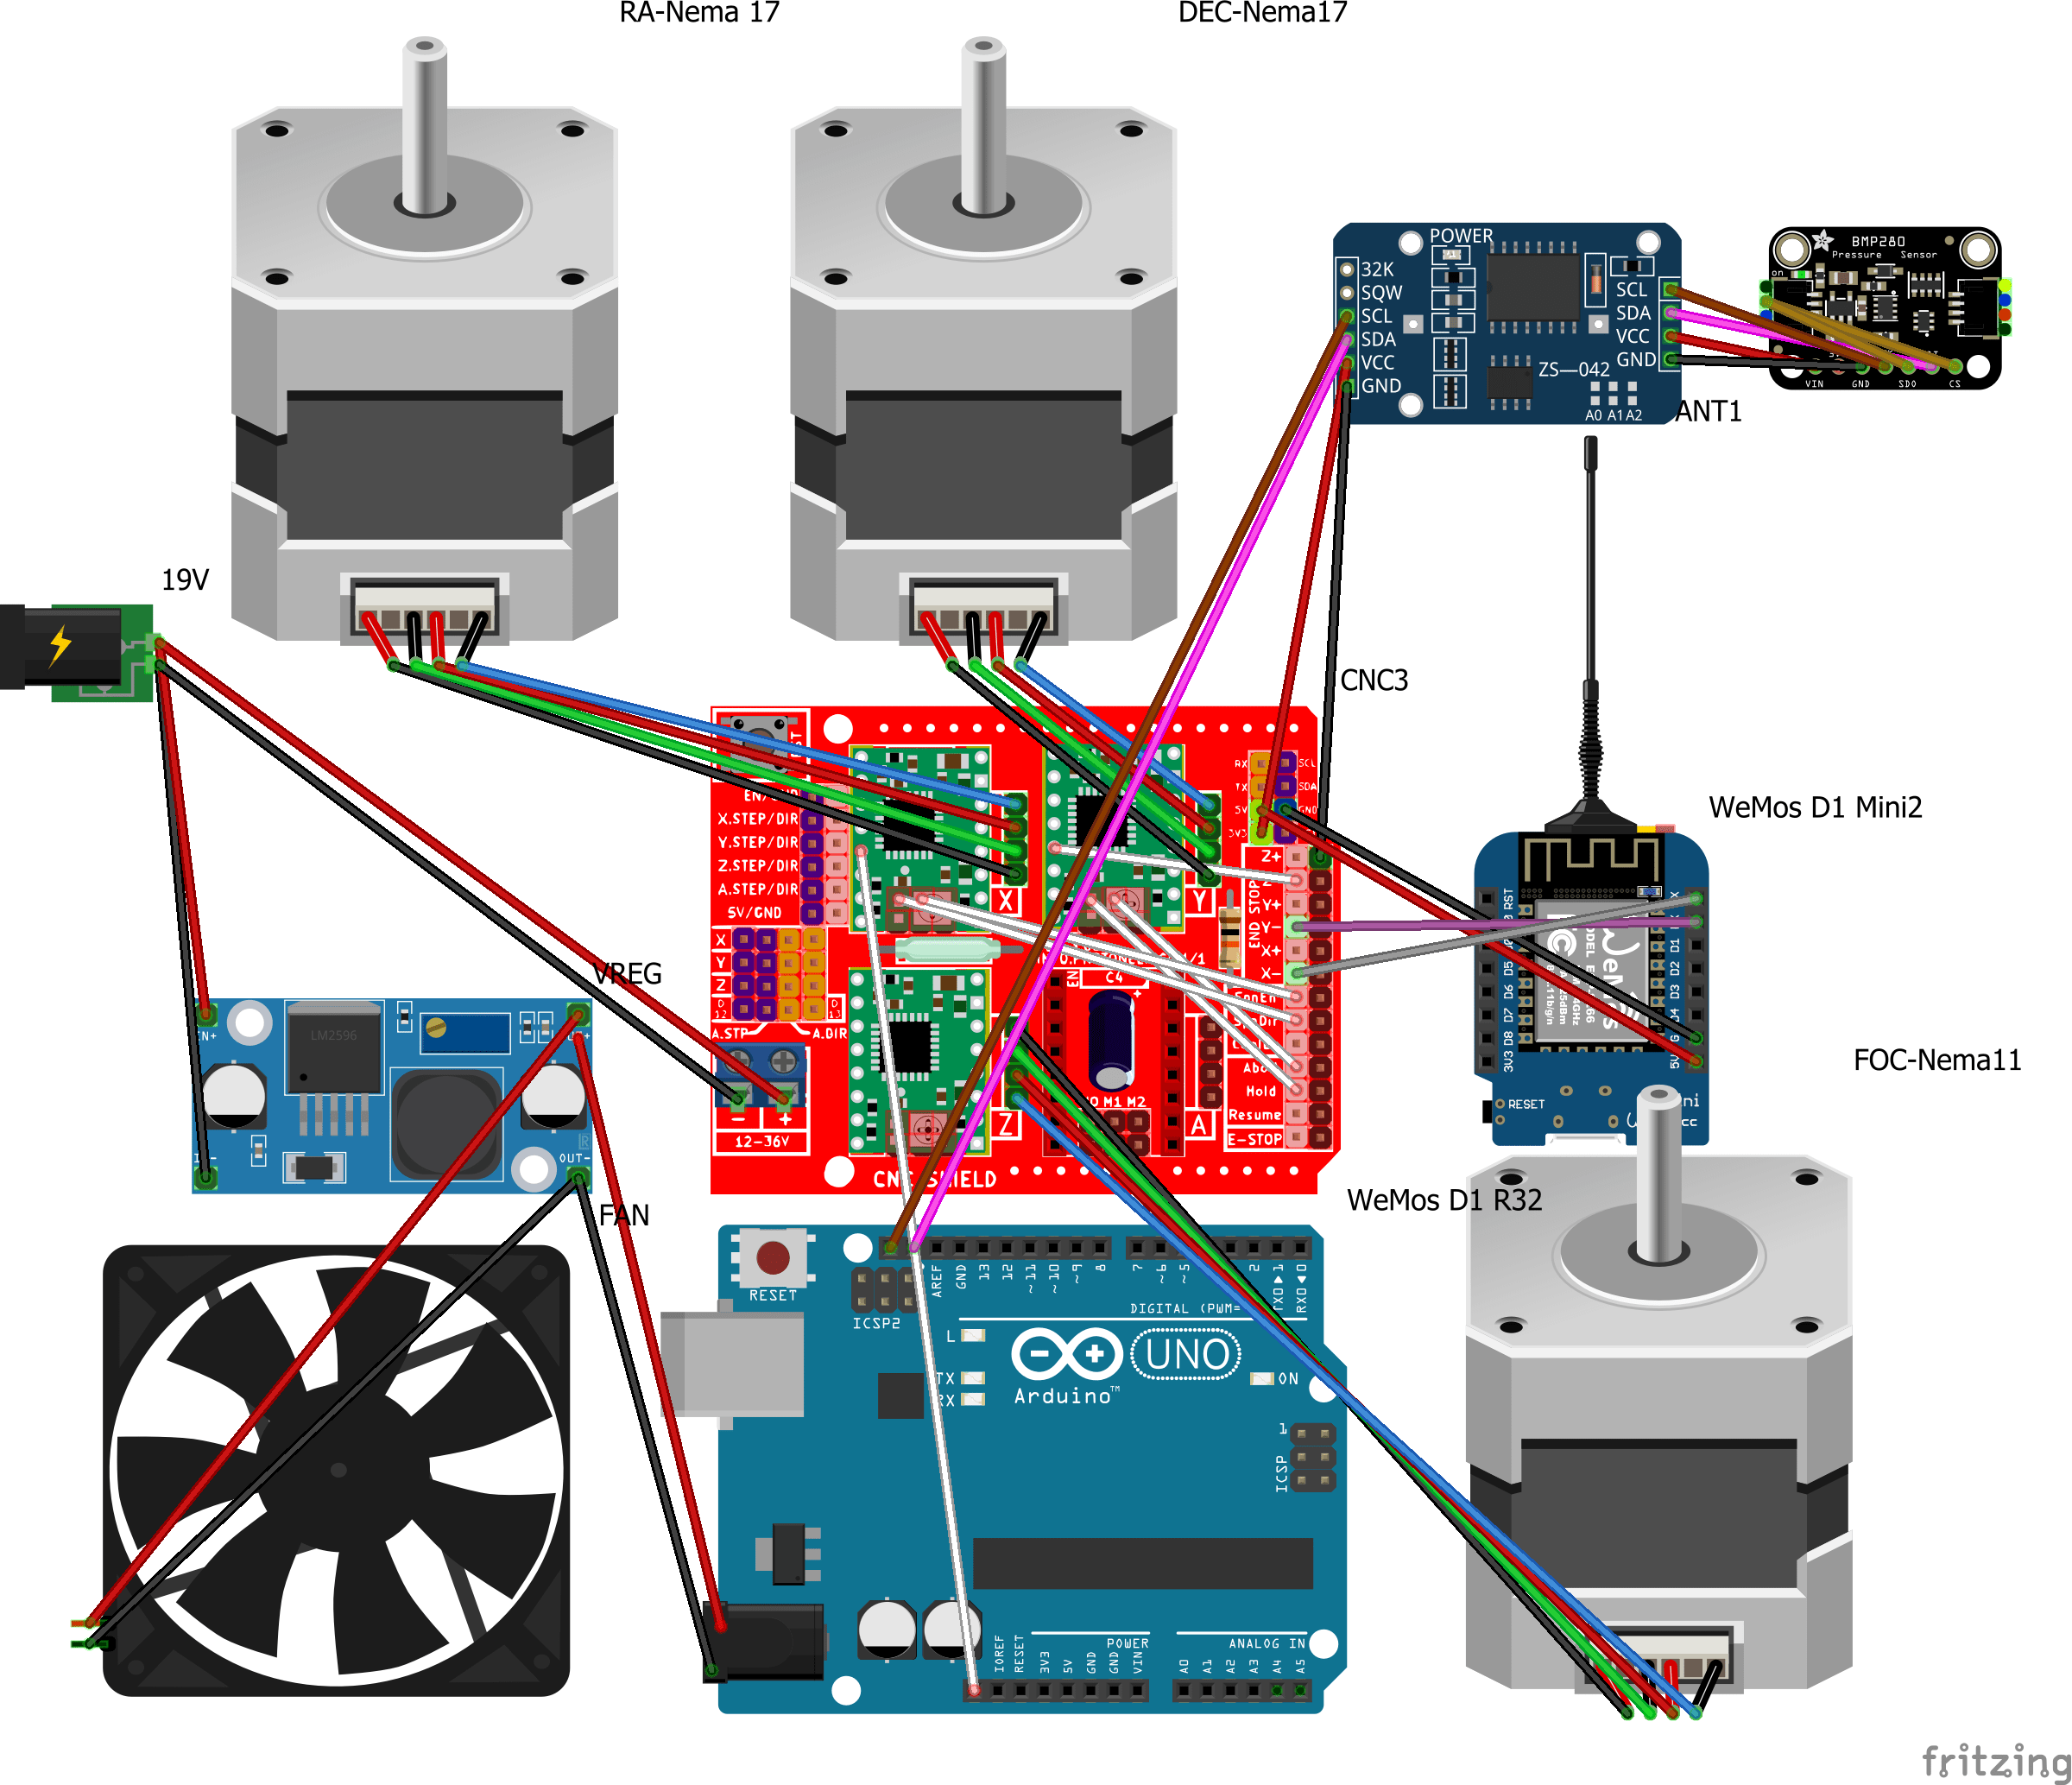
\includegraphics[scale=0.5]{Fritzing/circuit-design_bb.png}
        \subcaption{Circuit design. \href{https://github.com/sebastiano123-c/Motorize-a-1980-telescope/blob/main/Setup/circuit-design_bb.png}{Here} can be found the png file.}
        \label{fig:circuit-design}
    \end{minipage}
    \caption{Main board components: (a) WeMos D1 R32 ESP32 board, (b) CNC shield V3 and (c) the circuit design: the Arduino board is instead a ESP32 board, like the one of figure (a); the white cables are our modifications on the board.}
    \label{fig:electronics}
\end{figure*}

% \begin{figure*}
%     \begin{subfigure}[t!]{.25\textwidth}
%         \centering
%         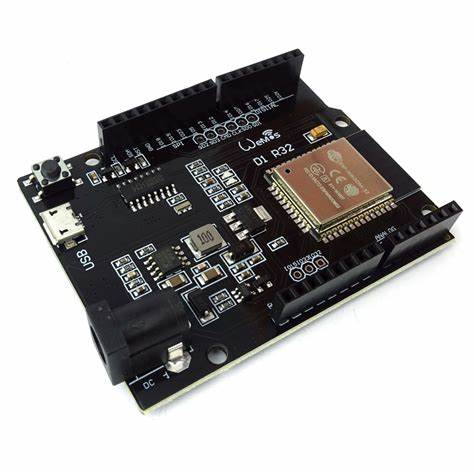
\includegraphics[scale=0.28]{esp32_d1_r32.jpg}
%         \caption{ESP32 D1 R32 picture.}
%         \label{fig:esp32}
%     \end{subfigure}
%     \begin{subfigure}[t!]{0.25\textwidth}
%         \centering
%         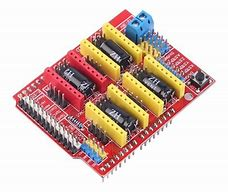
\includegraphics[scale=0.5]{CNC3.jpg}
%         \caption{CNC3 Shield V3.}
%         \label{fig:cnc3}
%     \end{subfigure}
%     \begin{subfigure}[t!]{0.5\textwidth}
%         \centering
%         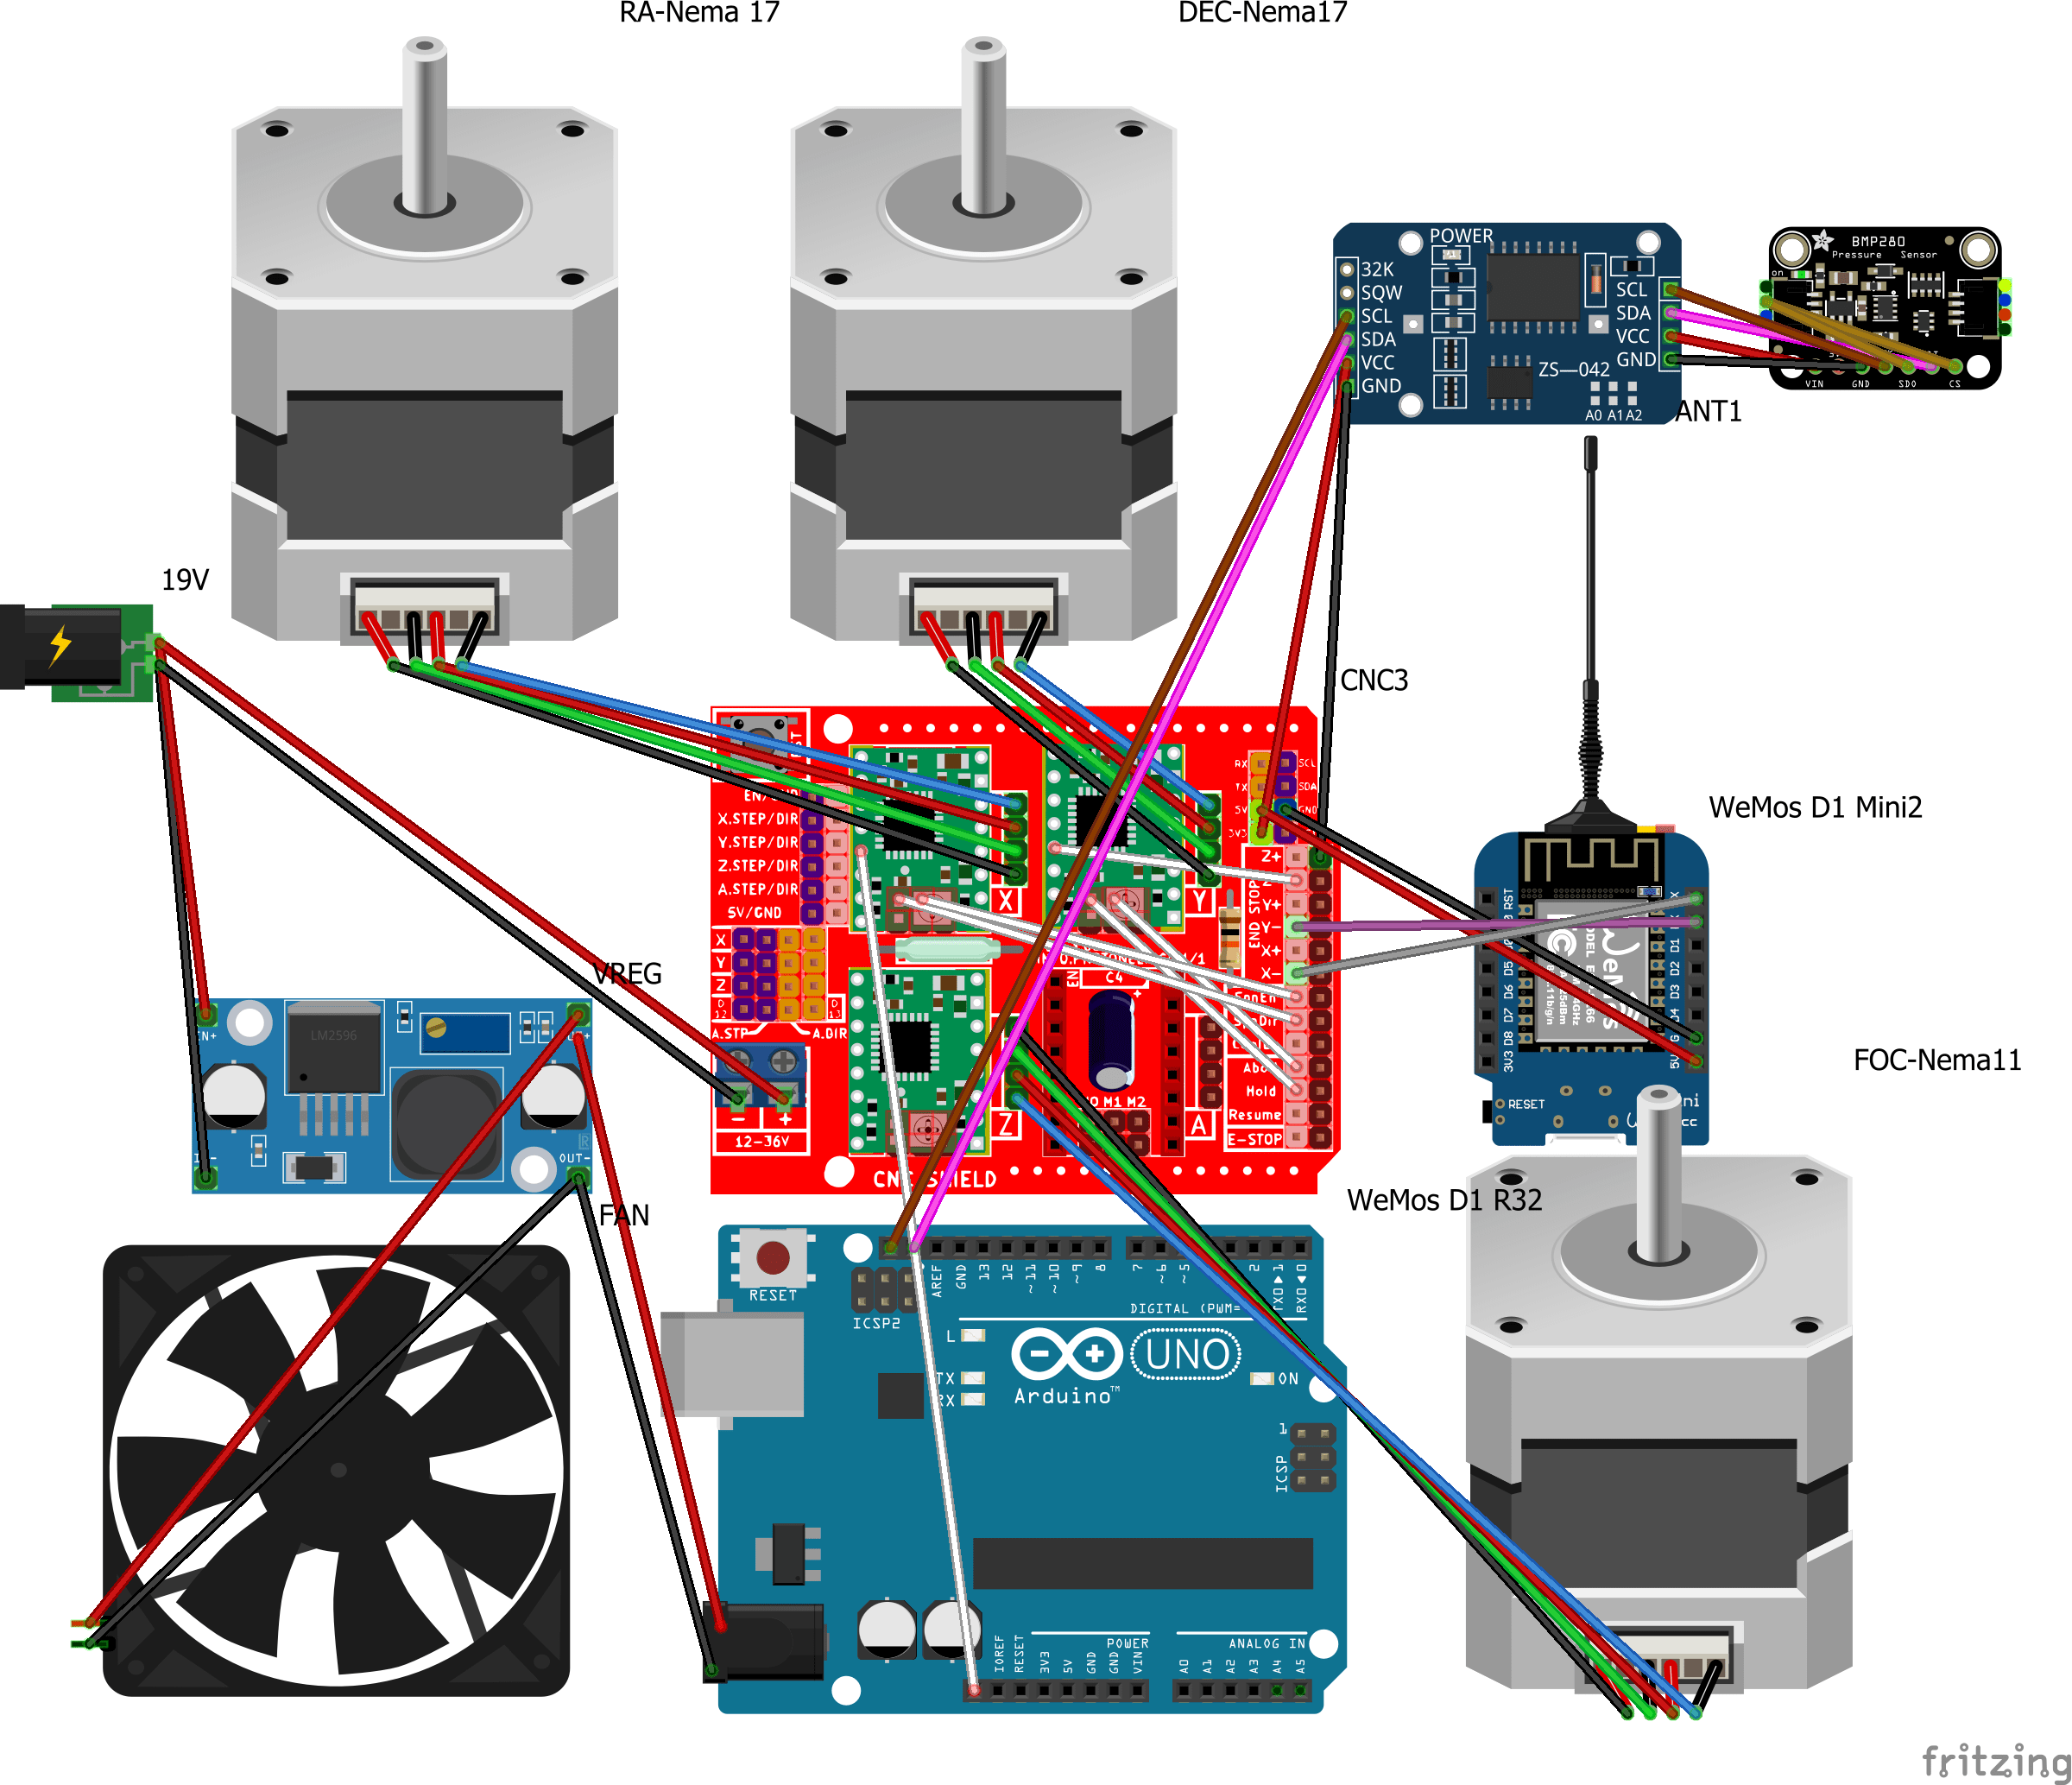
\includegraphics[scale=0.5]{Fritzing/circuit-design_bb.png}
%         \caption{Circuit design.}
%         \label{fig:circuit-design}
%     \end{subfigure}
%     \caption{Main board components: (a) WeMos D1 R32 ESP32 board and (b) CNC shield V3.}
%     \label{fig:electronics}
% \end{figure*}

\subsection{CNC Shield V3}
To better optimize space and wires connections, we have bought a CNC Shield V3 (a.k.a. CNC3), see figure \ref{fig:cnc3}.

It is a printed circuit board (PCB) built for 3D printers.
The shield is attached directly above the ESP32.
It has four slots, each one can host a motor driver, thus using this shield there can be handled four stepper motors: RA and DEC motors, first focuser and photography rotator or second focuser.

This shield can be "manipulated" to obtain better performances.

\subsection{Motor drivers}
A stepper motors works only with a driver chip that controls the motor movements.
Three types of drivers have been used during the configuration of the setup.
\begin{enumerate}
    \item DRV8825;
    \item TMC2209;
    \item TMC2208.
\end{enumerate}

In each driver the right amount of current is set, otherwise the stepper motor could work improperly.
This current depends on the stepper motor current per phase parameter.
Typically, drivers have a tunable screw for the tension \(V_{ref}\).
For each type of driver, the formula to calculate the tension \(V_{ref}\) depending on the current/phase are different.\footnote{See \href{https://all3dp.com/2/vref-calculator-tmc2209-tmc2208-a4988/}{this} for more details.}

The procedure is the following:
\begin{itemize}
    \item rotate the screw in the counter clock direction;
    \item using a multimeter, check that the tension is zero;
    \item slightly rotate the screw until the tension is the desired one.
\end{itemize}
We recommend reducing the theoretical value by a 10\%-30\% to prevent motor dangers.

\subsubsection{DRV8825}
For these drivers the tension to be set is roughly the half of the value of the nominal current/phase of the motor.
For example, if the motor has a current/phase \(1\)A, the tension would be \(0.5\)V.
\\
\\
\begin{minipage}
    {.4\textwidth}
    \centering
    \begin{tabular}{cc}
        \hline
        \textbf{Current phaser (A)} & \textbf{Current (A)} \\
        \hline
        0.90 & 0.45 \\
        2.00 & 0.90             
    \end{tabular}
    \captionof{table}{DRV8828 drivers setup current. Note that we have set a value smaller than the one calculated to prevent motor to break.}
    \label{tab:drivers_curr}
\end{minipage} 

\subsubsection{TMC2208 and TMC2209}
For these drivers the tension value is roughly the same of the current/phase value, \textit{e.g.} if \(I=1\)A the tension would be \(V_{ref}=1\)V.
Be aware that the TMC2208 has a maximum current output of 1.2A.

The calculation is 
\[\frac{I}{\sqrt{2}}=\frac{325mV}{110m\Omega+20m\Omega}\cdot\frac{1}{\sqrt{2}}\cdot\frac{V_{ref}}{2.5V}\Rightarrow V_{ref} = I \cdot 1\Omega.\]
Remember to reduce to value by a 10\%-30\%.

\begin{minipage}
    {.4\textwidth}
    \begin{tabular}{ccc}
       Driver & Current/phase (A) & Current (A) \\
        \hline
       TMC2208 & 0.90 & 0.81 \\
       TMC2208 & 2.00 & 1.63 \\                
       TMC2209 (focuser) & 0.67 & 0.50                
    \end{tabular}
    \captionof{table}{DRV8825 drivers setup current. Note that we have set a value smaller than the one calculated to prevent motor to break.}
    \label{tab:drivers_curr}
\end{minipage} 

\begin{figure*}
    \begin{subfigure}[t!]
        {0.33\textwidth}
        \centering
        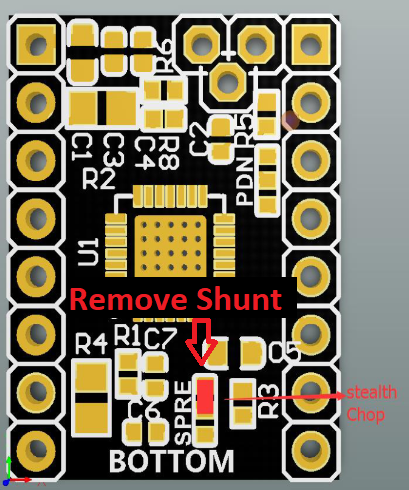
\includegraphics[scale=0.5]{TMC2209_Spread1.png}
        \caption{TMC2209 driver with highlighted modifications. }
        \label{fig:tmc-spread1}
    \end{subfigure}
    \begin{subfigure}[t!]
        {0.33\textwidth}
        \centering
        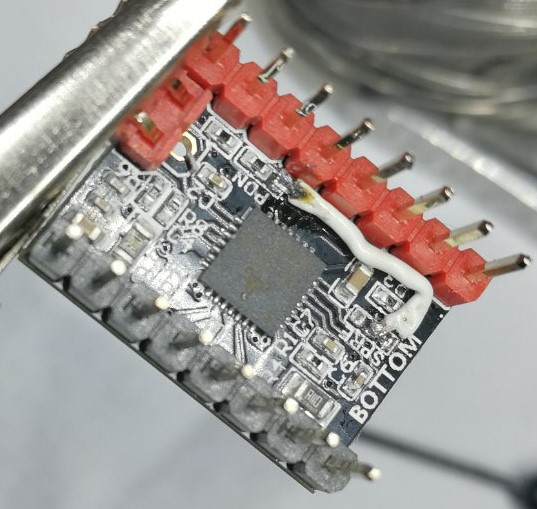
\includegraphics[scale=0.18]{TMC2209_Spread2.jpg}
        \caption{Connection of the Spread pin to pin 5 by wire.}
        \label{fig:tmc-spread2}
    \end{subfigure}
    \begin{subfigure}[t!]
        {0.33\textwidth}
        \centering
        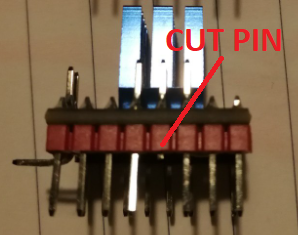
\includegraphics[scale=0.6]{TMC2209_Spread3.png}
        \captionof{figure}{ Cut low pin 5. }
        \label{fig:tmc-spread3}
    \end{subfigure}
    \caption{TMC2209 modifications.}
    \label{fig:cnc3-mod}    
\end{figure*}

\subsection{CNC3 and TMC2209 modifications}
CNC3 shield does non permit "on the fly" change of microstepping since they are achieved via the MS0\(/\)MS1\(/\)MS2 fixed jumpers below the motor drivers. This means that you cannot have different microstepping for tracking and slewing unless you use TMC2130 or TMC5160 through SPI interface. To overcome this CNC3 limit when using other drivers (\textit{e.g.} TMC2209 that are very silent, guarantee a 2A current per phase and are somehow cheap), it is necessary to do some soldering on the CNC3 and the TMC2209 and modify the pinmap "Pins.CNC3.h".
\subsubsection{Microsteps control}
First of all it is necessary to configure the TM2209 stepper driver (TMC2209 Bigtreetech v1.2) to remove the Spread shunt (that controls StealthChop vs SpreadCycle mode) on the TMC2209 board and then wire connect the Spread to pin 5 of J1, see figures \ref{fig:tmc-spread1} \ref{fig:tmc-spread2}.

Finally, you have to cut the low pin 5 of J1 on the TMC2209 driver since it is shortcutted with pin 6 (CLK) on the CNC3, see figure \ref{fig:tmc-spread3}.

At this point, we have a wire connected (some soldering) the MS0 and MS1 of Axis X to the SpnEn and SpnDir pins of CNC3 respectively. In the same way, we have a wire that connected the MS0 and MS1 of Axis Y to the HOLD and ABORT pins respectively. In this way, we are able, after modifying the pinmap in "Pins.CNC3.h" to control the microstepping in Tracking and Goto both in RA and DEC.
You can find the modified Pinmap "Pins.CNC3.h" \href{https://github.com/sebastiano123-c/Motorize-a-1980-telescope/blob/main/OnStep/src/pinmaps/Pins.CNC3.h}{here}.

The last modification is simply to connect with a wire jumper pin 5 of TMC2209 of AXIS X to the pin IO0 of the WeMos D1 R32 as well as connect pin 5 of TMC2209 of AXIS Y to the pin Z\(-\) of the CNC3.
With this done we able to set programmatically (via Config.h) the SpreadCycle (StealthChop) mode using the TMC2209\(\_\)QUIET (TMC2209\(\_\)VQUIET) constants.

\href{https://github.com/sebastiano123-c/Motorize-a-1980-telescope/blob/main/OnStep/Config.h}{Here} is the updated "Config.h".

\subsection{Power supply}
The power supply is provided by a 19V 5A power supply as in table \ref{tab:power_supply}.

\begin{minipage}
    {.4\textwidth}
    \begin{tabular}{cc}
         voltage output (V) & current output (A) \\
         \hline
        19.3 & 4.74 \\
    \end{tabular}
    \captionof{table}{Nominal tension and current outputs of the power supply.}
    \label{tab:power_supply}
\end{minipage}

For our initial purposes it was enough, indeed 5A are enough to feed quite well two stepper motors and a poor electronics.
A rough estimation poses 1.8A for DEC motor, 0.9A for RA motor and few milliampéres for the ESP32. 
The reader is strongly encouraged to check the total current its circuit needs before buying a power supply.

To provide the 3.3V tension to the microcontroller, a ICQUANZX voltage regulator is place between the power supply and the ESP32.

\subsection{Sensors: WiFi connection, Real time clock (RTC) and weather sensor (BMP280)}
OnStep contains the so-called Smart Web Server (SWS) that provides WiFi (or Ethernet) connections using an IP but it does not exploit the native ESP32 chip for the WiFi connection;
To command the mount via WiFi a ESP8688 WeMos D1 mini must be connected to the CNC3.\footnote{For the pinout maps look at this \href{https://onstep.groups.io/g/main/wiki/19670}{connection diagram}.}
Many devices support this type of connection including cell-phones, tablets, laptop/desktop computers, etc.
Using this library, it is possible to use programs such as Stellarium via ASCOM drivers provided by the \href{http://www.stellarjourney.com/index.php?r=site/software_telescope}{OnStep project}.
We have added an antenna to enhance the WiFi connection range.\footnote{Take a look at \href{https://www.instructables.com/External-Antenna-for-ESP8266/}{this} to see how to do that.}

The weather sensor BMP280 is modified as follows: the CSB and the SDO pins are connected directly to the Vcc.
The sensor is then attached directly to the RTC module Ds3231.

The RTC, BMP280, the WiFi module and the stepper motors are connected to the WeMos ESP32 D1 R32+CNC3 board as in figure \ref{fig:circuit-design}.
